\documentclass[../main.tex]{subfiles}
    
\begin{document}
The software is separated into modules according Figure [TBD], where the
program is launched from “main()”. The separation of modules of different
purpose allows for improving the software by focusing only one part of the
program. Some of the modules are just a wrapper for an API, which may be
implemented from scratch in the future. The purpose of the wrapper is to allow
the from-scratch-implementations, without rewriting the code for the module
using the API (e.g. without changing main to implement Text-to-Speech from
scratch).

\begin{figure}[h]
  \centering
  \caption{An UML of the software.\label{fig:main_uml}}
  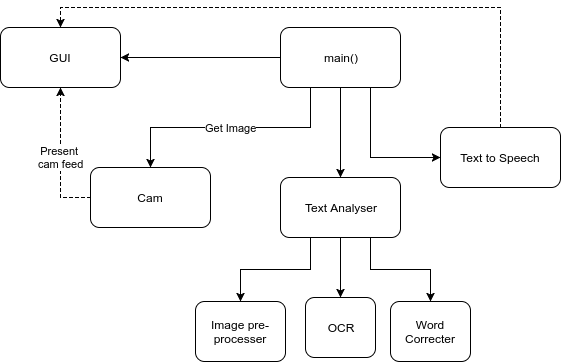
\includegraphics[width=1.0\textwidth]{res/UML1}
\end{figure}

\subsection{GUI}
The graphical interface consists of a windows with various options. It
displays live camera feed and giving options to the user to capture an image
by pressing a button. It has a text field which contains the text after an
image has been analyzed. To be able to implement the camera, OpenCV are used.
The other graphical components are Tkinter objects.

\subsection{Optical character recognition --- OCR}
OCR is the module that turns an image into characters. It is a wrapper for the
Tesseract API, which is a  machine learning-based open source OCR engine that
is maintained by Google. OCR may be implemented from scratch in the future,
using Neural Networks.

\subsection{Text-To-Speech}
TTS is the module that turns text (given from OCR) into speech. The module is
a wrapper for gTTS, which is an interface for Google’s Text-To-Speech API.

\subsection{Tests}
\textit{TBD}
\end{document}